%! Tex program = xelatex   
\documentclass{article}
\usepackage{graphicx,subfig}
\usepackage[left=2cm, right=2cm, lines=45, top=0.8in, bottom=0.7in]{geometry}
\usepackage{xeCJK}
\usepackage{amsmath}
\usepackage{booktabs} %表格
\usepackage{tikz}
\usepackage{graphics}
\usepackage{xcolor} 
\usepackage{tikz} 
\usepackage{svg}
\usetikzlibrary{arrows,shapes,chains}
\setmainfont{Times New Roman}
\setCJKmainfont{Songti SC}
\setCJKfamilyfont{song}{Songti SC}
\renewcommand{\baselinestretch}{1.5} %行间距
%-----------------------伪代码------------------
\usepackage{algorithm}  
\usepackage{algorithmicx}  
\usepackage{algpseudocode}  
\floatname{algorithm}{Algorithm}  
\renewcommand{\algorithmicrequire}{\textbf{Input:}}  
\renewcommand{\algorithmicensure}{\textbf{Output:}} 
\usepackage{lipsum}  
\makeatletter
\newenvironment{breakablealgorithm}
  {% \begin{breakablealgorithm}
  \begin{center}
     \refstepcounter{algorithm}% New algorithm
     \hrule height.8pt depth0pt \kern2pt% \@fs@pre for \@fs@ruled
     \renewcommand{\caption}[2][\relax]{% Make a new \caption
      {\raggedright\textbf{\ALG@name~\thealgorithm} ##2\par}%
      \ifx\relax##1\relax % #1 is \relax
         \addcontentsline{loa}{algorithm}{\protect\numberline{\thealgorithm}##2}%
      \else % #1 is not \relax
         \addcontentsline{loa}{algorithm}{\protect\numberline{\thealgorithm}##1}%
      \fi
      \kern2pt\hrule\kern2pt
     }
  }{% \end{breakablealgorithm}
     \kern2pt\hrule\relax% \@fs@post for \@fs@ruled
  \end{center}
  }
\makeatother
%------------------------代码-------------------
\usepackage{xcolor} 
\usepackage{listings} 
\usepackage{fontspec}
\newfontfamily\menlo{Menlo}
\setmonofont[Mapping={}]{Monaco} 
\definecolor{mygreen}{rgb}{0,0.6,0}
\definecolor{mygray}{rgb}{0.5,0.5,0.5}
\definecolor{mymauve}{rgb}{0.58,0,0.82}
\lstset{ %
backgroundcolor=\color{white},   % choose the background color
basicstyle=\footnotesize\ttfamily,        % size of fonts used for the code
columns=fullflexible,
breaklines=true,                 % automatic line breaking only at whitespace
captionpos=b,                    % sets the caption-position to bottom
tabsize=4,
commentstyle=\color{mygreen},    % comment style
escapeinside={\%*}{*)},          % if you want to add LaTeX within your code
keywordstyle=\color{blue},       % keyword style
stringstyle=\color{mymauve}\ttfamily,     % string literal style
frame=single,
rulesepcolor=\color{red!20!green!20!blue!20},
numbers=left,
 numberstyle=\tiny\menlo
% identifierstyle=\color{red},
% language=c++,
}
\begin{document}
\title{生成对抗网络实验报告}
\author{朱浩泽 1911530}
\maketitle
\section{网络结构}
\large
\begin{lstlisting}
Discriminator(
   (fc1): Linear(in_features=784, out_features=128, bias=True)
   (nonlin1): LeakyReLU(negative_slope=0.2)
   (fc2): Linear(in_features=128, out_features=1, bias=True)
)   

Generator(
  (fc1): Linear(in_features=100, out_features=128, bias=True)
  (nonlin1): LeakyReLU(negative_slope=0.2)
  (fc2): Linear(in_features=128, out_features=784, bias=True)
)
\end{lstlisting}
\section{实验结果}
\subsection{训练损失函数曲线}
\begin{figure}[H]
   \centering
   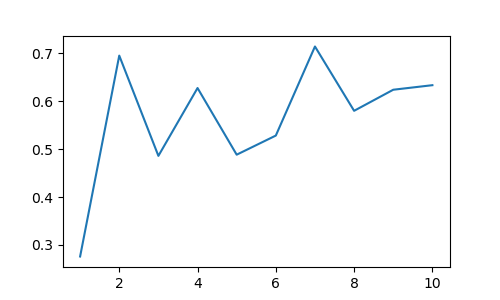
\includegraphics[scale = 0.75]{lossG.png}
   \caption{\textbf{生成器的损失函数曲线}}
\end{figure}
\begin{figure}[H]
   \centering
   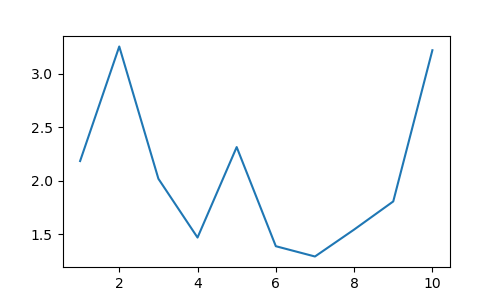
\includegraphics[scale = 0.75]{lossV.png}
   \caption{\textbf{判别器的损失函数曲线}}
\end{figure}
gan是个minimax game,生成器和判别器一直在进行对抗,所以loss应该是很杂乱,一会上升一会下降。这就是gan难以训练的原因,我们不太能通过查看loss来说明gan训练得怎么样。

\subsection{自定义一组随机数,生成8张图}
\begin{figure}[H]
   \centering
   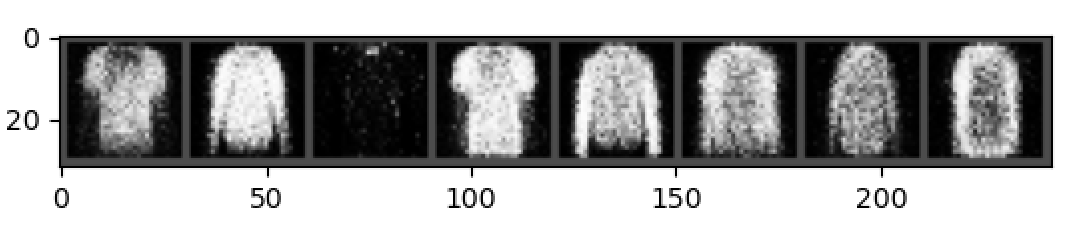
\includegraphics[scale = 0.75]{11.png}
   \caption{\textbf{利用随机数生成的8张图片}}
\end{figure}
\subsection{针对自定义的100个随机数,自由挑选5个随机数,查看调整每个随机数时,生成图像的变化(每个随机数调整3次,共生成15x8张图),总结调整每个随机数时,生成图像发生的变化。}
为了方便我们画图,我们进行了如下操作,首先利用 \lstinline{fixed_noise = torch.randn(8, 100, device=args.device)}生成了八个100维的随机数,作为生成图像使用的随机数。然后我们利用 \lstinline[]{fixed_noise = fixed_noise.repeat(5, 1)}将这八个随机数分被复制五分,作为我们要更改的每五个位置。我们对于一行中的八个随机数图像,在一次实验中更改的随机数的位置相同,每次实验更改的随机数数值相同。所以一次实验可以画出一张$8\times 5$的图。每张图的第一行代表的是更改第一个位置的随机数,第二行是代表更改第20个位置的随机数,第三行代表的是更改第40个位置的随机数,第四行是代表第60个位置的随机数,最后一行代表的是更改第80个位置的随机数。

\begin{figure}[H]
   \centering
   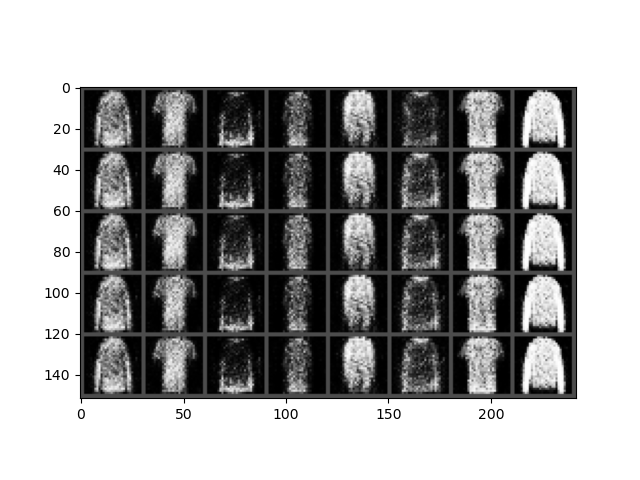
\includegraphics[scale = 0.5]{1:2.png}
   \caption{\textbf{将随机数指定为0.5}}
\end{figure}
\begin{figure}[H]
   \centering
   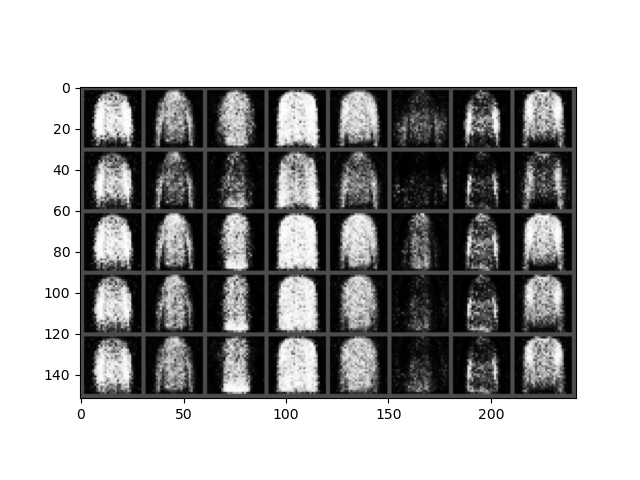
\includegraphics[scale = 0.5]{3.png}
   \caption{\textbf{将随机数指定为3}}
\end{figure}
\begin{figure}[H]
   \centering
   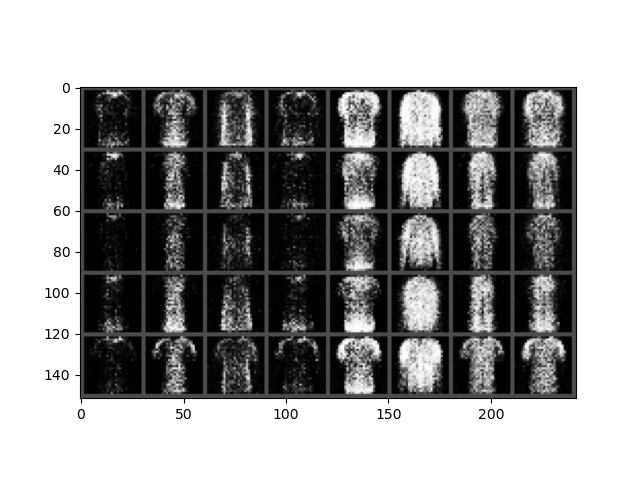
\includegraphics[scale = 0.5]{10.png}
   \caption{\textbf{将随机数指定为10}}
\end{figure}
首先我们观察可以看出,当随机数设定的较小的时候(如0.3),在不同位置改变一个这样的小随机数,收获的效果是比较小的,甚至可以说基本没有什么肉眼可以观察出来的变化;但是,当随机数设置的较大的时候(如10),如果我们在不同位置改变一个这样的小随机数,收获的效果还是比较明显的,可以很清晰的从最后一张图上看出,相对于位置60变为10,位置80的改变直接让裤子变成了两件衣服。当我们在观察相同位置的随机数改变时,我们发现,过小的随机数(0.3)或者过大的随机数(10)都会导致生成的图像的亮度较低,甚至有些图片接近于全黑,而当我们使用一个适中的随机数的时候,我们的模型生成的效果相对来说较为明亮,且生成的图像的效果较好。
\end{document}
